% methods.tex
% Author: Tony Kabilan Okeke
% Date: 2023-03-23

\section{Methods}

We used the `limma' R package \cite{limma} to perform differential expression analysis
on each of the 7,130 mouse RNA-seq datasets based on the metadata downloaded from GEO.
We extracted the log2 fold change (logFC) values for all genes and combined them into a
feature matrix. We then performed Gene Ontology (GO) enrichment analysis on the
differentially expressed genes using the `GOfuncR' R package \cite{GOfuncR}. The
significantly enriched GO terms ($p < 0.05$) were combined into a single matrix and were
one-hot encoded to be used as features for the classification model. Finally, we
normalized the feature matrix using the `StandardScaler' function from `Scikit-Learn'
\cite{sklearn}, which transforms the data to have zero mean and unit variance. The
dataset was then split into a training, validation and test sets with 70\%, 15\%, and
15\% of the data, respectively.

\vspace{0.2cm}

We used `VarianceThreshold' from `Scikit-Learn' \cite{sklearn} to remove low-variance
genes from the data, leaving 21,953 genes in the feature matrix. We then visualized the
data using PCA and t-SNE with 2 components each. PCA is a linear technique that preserves
the maximum variance of the data, while t-SNE is a non-linear technique that preserves
the local structure of the data.

\vspace{0.2cm}

We built a simple autoencoder using the `Keras' library with `TensorFlow' as the backend
\cite{tensorflow}. The autoencoder consisted of a fully connected, feed-forward neural
network with one hidden layer and 2000 neurons. The hidden layer had a rectified linear
unit (ReLU) activation function, while the output layer had a sigmoid activation function.
We trained the autoencoder using the `Adam' optimizer with a learning rate of 0.001 and a
batch size of 128. The loss function was the mean squared error between the input and
output. We trained the model to reconstruct the feature matrix (logFC values) for 50
epochs and evaluated its performance by calculating the loss on the validation set.
Figure \ref{fig:architecture} shows the architecture of the autoencoder. To identify the
optimal number of hidden layers and neurons, we performed a random search over the
hyperparameter space. We also used the `reduceLRonPlateau' callback to reduce the
learning rate by a factor of 0.5 when the validation loss did not improve for 5
consecutive epochs. The model's performance was evaluated using the cross-validation
loss on the validation set. The model was implemented in Python 3.9.16 through Google
Colaboratory.

    {
        \centering
        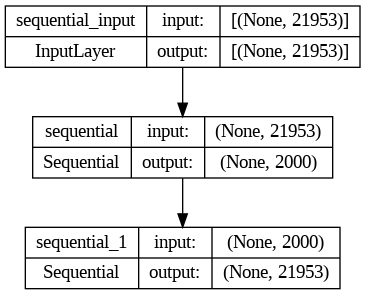
\includegraphics[width=.65\columnwidth]{./images/model.png}
        \captionof{figure}{Architecture of the autoencoder model.}
        \label{fig:architecture}
    }
